\section{Implementation Details}
\subsection{Object Proposals}
We use MCG object proposals in~\cite{arbelaez2014multiscale} as object candidates. Since the object proposals mainly covers the objects,  we also generate a small number (20$\sim$30 per image) of segments using the stable segmentation algorithm from~\cite{chen2011piecing} to cover the whole scene including contextual classes. To reduce the computational overhead, our context voting step uses only the stable segments. The stable segmentation gives a coarse level of object/context division and reduces the computational complexity of context voting compared to the large number of finer object proposals, while still maintaining a semantically informative contextual inference. 

\subsection{Datasets}
We conduct our training and experiments on the Pascal VOC dataset.~\cite{Everingham10} which is a \textit{de facto} benchmark for object detection. Since the original dataset does not provide annotation of segmentation and contextual classes, we train our policy using the Pascal Context dataset~\cite{mottaghi2014role} which fully annotates every pixel of the Pascal VOC 2010 train and validation sets, with additional contextual classes such as sky, grass, ground, building etc., which is adequate for our purposes. We use the 33 context classes from~\cite{mottaghi2014role} and train our policy on the Pascal Context training set, and test our algorithm and baselines on the validation set. We also test our policy on the MSRC dataset~\cite{shotton2006textonboost} to show our algorithm can generalize to different data. 

\subsection{Feature Representation}
To classify object proposals, we extract region features and classify them using the deep neural network model in~\cite{BharathECCV2014} fine-tuned on Pascal VOC 2012. For the policy action classifiers, we also use the same model to extract features for states represented by the masks of search area $X^t$ and observed area $O^t$ in state $s_t$, then concatenate the features as inputs to the policy. For context classifiers we use a subset of the appearance features for superpixels from~\cite{tighe2010superparsing} and learn one-vs-all SVM models for classification.

\section{Experiments}

We conduct our experiments on the Pascal VOC 2010 dataset, in consistence with the data to train our context model. We evaluate the object detection performance by mean average precision (mAP). Since we also evaluate the performance of simultaneous detection and segmentation, we use the validation set as our test set which provides object segmentation annotations. 

%\subsection{Reduction of Number of Object Proposals}

\begin{figure}[htb!]
\begin{center}
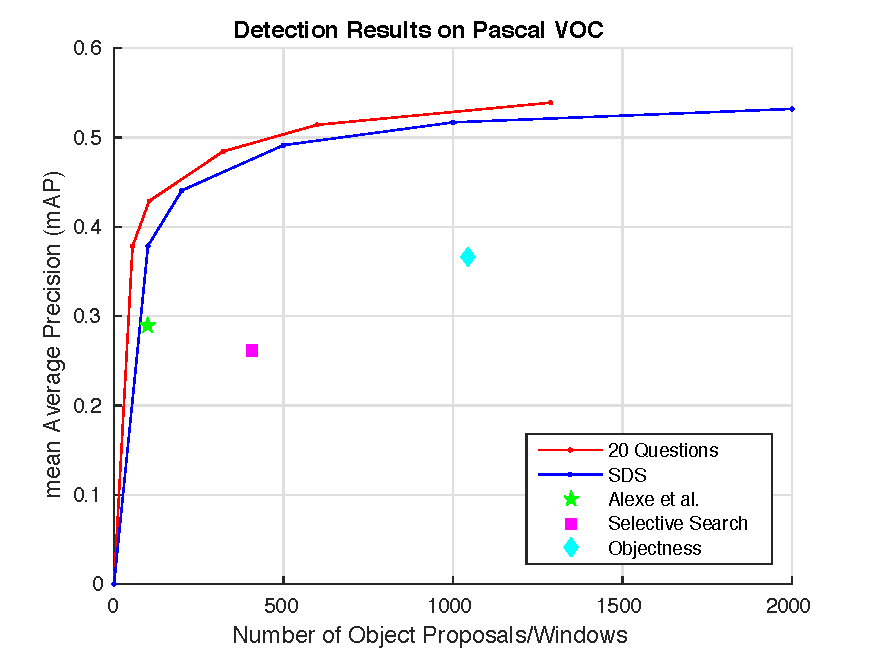
\includegraphics[width=0.6\linewidth]{figures/numprop.pdf}
\end{center}
\caption{Performance on Pascal VOC dataset. Best viewed in color. }
\label{fig:mapVSnumprop}
\end{figure}

%%%%%%%%%%%%%%%%%%%%%%%%%%%%%%%%%%%
\subsection{Reduction of Object Proposals} 
Figure~\ref{fig:mapVSnumprop} shows the average precision performance on the Pascal VOC 2010 dataset with respect to the number of object proposals/windows used. We compared our 20 question approach to the baseline of running detectors in~\cite{BharathECCV2014} exhaustively over all object proposals,  window selection driven by context in~\cite{bogdan2012context}, detection using object proposals in selective search~\cite{van2011segmentation} and objectness~\cite{alexe2010object}. We can see that that our 20 questions detection algorithm can effectively reduce a large amount of object proposals ($30\% \sim 40\%$) with comparable performance to exhaustive detection on all object proposals. With the number of object proposals increasing, With the increase of the number of object proposals, our algorithm can even achieve results better than exhaustive methods due to the reduction of false positives. We can also see that with the same number of object proposals, our approach performs much more effectively by a large margin compared with random search approach which randomly samples the same number of object proposals for detection. 

%%%%%%%%%%%%%%%%%%%%%%%%%%%%%%%%%%%%%

\subsection{Performance of Object Detection} We compare our model with current state-of-the-art exhaustive search baselines SDS~\cite{BharathECCV2014} and RCNN~\cite{girshick14CVPR}, as well as  a recent proposed contextual model in~\cite{mottaghi2014role}, which considers global and local context in a Markov Random Field framework based on deformable part-based model. This model has high computational cost since it needs to evaluate hundreds of thousands of windows as well as the context deformation term between all context boxes in the graph. Table~\ref{Tablepascal} shows the classwise mAP of our 20 questions-based object detection with other context based methods and their corresponding baselines.  Our 20 question detection approach has outperformed the SDS and RCNN exhaustive search baselines as well as DPM based context approaches. Both the SDS and the 20 question method starts with 2000 object proposals per image; after the 20 questions refinement of the search space the average number of detector evaluations (including the overhead of context classifiers evaluated) has decreased 36\%. We can see that although the performance for some classes have dropped due to possible rejection of true object candidates, more classes that are usually more correlated  to other objects in the scenes have significant gain over exhaustive search, such as boat, car, chair, cow, sofa etc., thus improving the overall average precision. 


\begin{table*}\tiny
\caption{Avg. Precision for detection of our algorithm against previous contextual approaches on PASCAL VOC10 dataset.}
\begin{tabular}{p{1.60cm}|p{0.144cm}p{0.144cm}p{0.144cm}p{0.144cm}p{0.144cm}p{0.144cm}p{0.144cm}p{0.144cm}p{0.144cm}p{0.144cm}p{0.144cm}p{0.144cm}p{0.144cm}p{0.144cm}p{0.144cm}p{0.144cm}p{0.144cm}p{0.144cm}p{0.144cm}p{0.144cm}p{0.144cm}c}
&{\begin{sideways}Aeroplane\end{sideways}}&{\begin{sideways}Bicycle\end{sideways}}&
{\begin{sideways}Bird\end{sideways}}&{\begin{sideways}Boat\end{sideways}}&{\begin{sideways}Bottle\end{sideways}}&{\begin{sideways}Bus\end{sideways}}
&{\begin{sideways}Car\end{sideways}}&{\begin{sideways}Cat\end{sideways}}&{\begin{sideways}Chair\end{sideways}}&{\begin{sideways}Cow\end{sideways}}
&{\begin{sideways}Dining Table\end{sideways}}&{\begin{sideways}Dog\end{sideways}}&{\begin{sideways}Horse\end{sideways}}&{\begin{sideways}Motor Bike\end{sideways}}&{\begin{sideways}Person\end{sideways}}
&{\begin{sideways}Potted Plant\end{sideways}}&{\begin{sideways}Sheep\end{sideways}}&{\begin{sideways}Sofa\end{sideways}}&{\begin{sideways}Train\end{sideways}}&{\begin{sideways}TV/Monitor\end{sideways}}
&{\begin{sideways}Average\end{sideways}}\\
DPM & 44.3 & 51.3 & 7.1 & 8.0 & 21.8 & 56.0 & 41.2 & 18.4 & 13.8 & 11.7 & 10.4 & 13.5 & 38.3 & 42.7 & 44.6 & 3.7 & 27.0 & 24.3 & 38.0 & 32.2 & 27.4 \\                                  
\hline                                                                                                                                                                                  
DPM + 33 Context & 46.4 & 50.8 & 7.5 & 8.2 & 21.2 & 55.3 & 41.6 & 20.0 & 14.7 & 11.8 & 11.6 & 13.9 & 37.9 & 40.2 & 45.1 & 4.2 & 24.1 & 27.6 & 40.8 & 33.9 & 27.8 \\                     
\hline                                                                                                                                                                                  
~\cite{mottaghi2014role}+20 Context & 46.9 & 50.1 & 9.2 & 9.5 & 30.1 & 57.2 & 44.1 & 30.7 & 12.7 & 15.1 & 12.9 & 14.2 & 35.6 & 44.8 & 44.0 & 4.9 & 30.6 & 20.1 & 42.2 & 34.8 & 29.5 \\  
\hline                                                                                                                                                                                  
~\cite{mottaghi2014role}+33 Context & 49.8 & 48.8 & 12.0 & 10.8 & 29.1 & 55.2 & 45.6 & 32.0 & 14.2 & 12.6 & 13.7 & 16.6 & 39.8 & 44.2 & 45.1 & 8.2 & 35.3 & 26.0 & 42.3 & 34.3 & 30.8 \\
\hline                   
RCNN~\cite{girshick14CVPR} &{\bf69.9} & 64.2 & 48.0 & 30.2 & 26.9 & 63.3 & 56.0 & 67.6 & 26.8 & 44.7 & 29.6 & 61.7 & 55.7 & {\bf69.8} & 56.4 & 26.6 & 56.7 & 35.6 & 54.4 & {\bf57.7} & 50.1\\                                                                                                                                                               
\hline  
SDS~\cite{BharathECCV2014} & 67.3 & 63.6 & 47.1 & 33.1 & {\bf34.3} & 67.2 & 55.8 & {\bf74.6} & 24.9 & 44.8 & 35.7 & {\bf62.7} & 62.5 & 64.8 & {\bf59.1} & {\bf26.9} & 54.2 & 40.7 & 61.3 & {55.7} & 51.8 \\        
\hline                                                                                                                                                                                  
SDS+20Q          & 66.8 & {\bf64.3} & {\bf48.9} & {\bf36.1} & 32.2 & {\bf67.7} & {\bf56.5} & 70.4 & {\bf28.1} & {\bf58.3} & {\bf37.2} & 60.5 & {\bf64.7} & 65.9 & 52.1 & 26.7 & {\bf57.8} & {\bf46.6} & {\bf62.9} & 53.3 & {\bf52.9} \\                           
\hline    
\end{tabular}
\label{Tablepascal}
\end{table*}
%%%%%%%%%%%%%%%%%%%%%%%%%%%%%%%%%%%%%
\subsection{Improvement on the search space accuracy} To show the quality of our predicted search area, we evaluate the mean intersect vs. union (IU) of the search area produced by our 20 questions approach with the groundtruth object. We also compare with the search area of the original detector, produced by the union of the object proposals with high scores. Table~\ref{tab:space} shows that our approach has significantly improved the accuracy of overlapping between the predicted search area and the target query object.  We also find that the mean IU of the 20 questions search space has come close to that predicted by the oracle trajectory, which shows that our imitation learning has learn a good policy that closely mimic oracle's behavior.
\begin{table}\scriptsize                               
\begin{center}
\begin{tabular}{|c|c|c|c|c|}                    
\hline                                          
 & Original & 20Q  & Oracle \\          
\hline                                          
 Mean IU & 64.12 &  73.9 &  \textbf{78.2} \\        
\hline                                          
\end{tabular}     
\end{center}                              
\caption{Mean intersect VS union (IU) of the predicted search area and the groundtruth objects. }                        
\label{tab:space}                      
\end{table}  
%%%%%%%%%%%%%%%%%%%%%%%%%%%%%%%%%%%%%

\subsection{Simultaneous detection and segmentation}
Given we are using segment based object proposals generated by~\cite{arbelaez2014multiscale}, our detection system can also perform segmentation for the objects. We compare our algorithm with~\cite{BharathECCV2014} in  the simultaneous detection and segmentation task using the $AP^r$ metric proposed in the SDS paper. Table~\ref{tab:pascalseg} and Table~\ref{tab:msrc} show the performance on Pascal VOC10 dataset and the MSRC dataset respectively. We have outperformed the SDS approach on both datasets, showing our 20 questions algorithm can generalize well from the detection to segmentation task, as well as generalize to other data such as MSRC.





\begin{table*}\tiny
\caption{AP$^r$ performance on PASCAL VOC10 dataset.}
\begin{tabular}{p{1.60cm}|p{0.144cm}p{0.144cm}p{0.144cm}p{0.144cm}p{0.144cm}p{0.144cm}p{0.144cm}p{0.144cm}p{0.144cm}p{0.144cm}p{0.144cm}p{0.144cm}p{0.144cm}p{0.144cm}p{0.144cm}p{0.144cm}p{0.144cm}p{0.144cm}p{0.144cm}p{0.144cm}p{0.144cm}c}
&{\begin{sideways}Aeroplane\end{sideways}}&{\begin{sideways}Bicycle\end{sideways}}&
{\begin{sideways}Bird\end{sideways}}&{\begin{sideways}Boat\end{sideways}}&{\begin{sideways}Bottle\end{sideways}}&{\begin{sideways}Bus\end{sideways}}
&{\begin{sideways}Car\end{sideways}}&{\begin{sideways}Cat\end{sideways}}&{\begin{sideways}Chair\end{sideways}}&{\begin{sideways}Cow\end{sideways}}
&{\begin{sideways}Dining Table\end{sideways}}&{\begin{sideways}Dog\end{sideways}}&{\begin{sideways}Horse\end{sideways}}&{\begin{sideways}Motor Bike\end{sideways}}&{\begin{sideways}Person\end{sideways}}
&{\begin{sideways}Potted Plant\end{sideways}}&{\begin{sideways}Sheep\end{sideways}}&{\begin{sideways}Sofa\end{sideways}}&{\begin{sideways}Train\end{sideways}}&{\begin{sideways}TV/Monitor\end{sideways}}
&{\begin{sideways}Average\end{sideways}}\\
\hline                                                                                                                                                                          
SDS~\cite{BharathECCV2014} &{\bf68.2} & 52.1 & 51.6 & 30.7 & {\bf34.2} & 66.7 & 52.4 & {\bf70.9} & 21.0 & 39.6 & 30.7 & {\bf58.8} & {\bf55.2} & {\bf54.0} & {\bf55.5} & 25.0 & 56.4 & 33.3 & 61.2 & {\bf58.4} & 48.8 \\
\hline                                                                                                                                                                          
SDS+20Q          & 66.7 & {\bf55.0} & {\bf52.2} & {\bf33.3} & 32.1 & {\bf67.2} & {\bf53.7} & 66.9 & {\bf24.2} & {\bf53.8} & {\bf32.0} & 56.9 & 54.1 & 53.3 & 49.6 & {\bf25.1} & {\bf58.1} &{\bf 35.1} & {\bf61.3} & 55.5 & {\bf49.3} \\                   
\hline     
\end{tabular}
\label{tab:pascalseg}
\end{table*}




\begin{table}\scriptsize                               
\begin{center}                                                                                                 
\begin{tabular}{|c|c|c|c|c|c|c|c|c|c|c|c|c|}                                                                     
\hline                                                                                                           
 & cow & sheep & bird & chair & cat & dog & boat & body & car & bike & plane & mean \\                           
\hline                                                                                                           
SDS~\cite{BharathECCV2014} & 87.4 & 87.6 & {\bf49.6} & {\bf52.2} & 75.0 & 72.3 & 49.2 & 62.5 & 73.0 & 80.7 & 93.8 & 71.9 \\
\hline                                                                                                           
SDS+20Q & {\bf88.4} & {\bf93.8} & 45.8 & 48.3 & {\bf82.6} & {\bf76.7} & {\bf51.7} & {\bf65.5} & {\bf79.0} & {\bf85.2} & {\bf95.7} & {\bf73.2} \\                   
\hline                                                                                                           
\end{tabular}                                                                                                 
\end{center}                              
\caption{AP$^r$ performance on MSRC dataset. }                        
\label{tab:msrc}                      
\end{table}                                                                                                    


% ferrarri 2012
% ~\cite{bogdan2012context} 25000 to 100 